\documentclass[a4paper,11pt]{report}
 
 \usepackage[left=3cm, right=3cm, top=3cm, bottom=3cm]{geometry}
\usepackage{graphicx}
\usepackage{listings}
\usepackage{titlesec}
\usepackage{fancyhdr}
\usepackage{epstopdf}
\usepackage{float}
\usepackage{amsmath}
\usepackage{setspace}
\usepackage{eufrak}
\usepackage{url}

\usepackage{courier}
 \newcommand{\textform}[1]{\fontsize{14}{20}\selectfont{#1}}
\pagestyle{fancy}
\fancyhf{}
\fancyhead[R]{\thepage}
\renewcommand{\chaptermark}[1]{\markboth{#1}{}}
\renewcommand{\headrulewidth}{1pt}
\renewcommand{\footrulewidth}{1pt}

\lhead{\footnotesize{FLIPPER ZERO
}}
\rhead{}
\lfoot{\footnotesize{Department of Computer Science \& Engg.}}
\cfoot{}
\rfoot{\thepage}

\titleformat{\chapter}[display]
{\normalfont\Large\bfseries\centering}{\chaptertitlename\
\thechapter}{20pt}{\Large}


%\title{\textbf{A seminar report on\\TRUSTWORTHINESS MANAGEMENT IN THE SOCIAL INTERNET OF THINGS} 
%}
%\author{\textbf{Deena Jose}}

\begin{document}

\thispagestyle{empty}
  \begin{center}
      \fontsize{22}{25}\selectfont{\textbf{GOVERNMENT POLYTECHNIC COLLEGE PERUMBAVOOR}}\\[.1cm]
            \fontsize{15}{25}\selectfont{\textbf{Koovappady P.O Ernakulam-683 544 Kerala
    }}\\[1.2cm]
    \begin{figure}[h]
	\centering
	\hspace{21pt}
	\includegraphics[width=.70\linewidth]{logo.png}
	\label{fig:logo.png}
\end{figure}
\fontsize{14}{25}\selectfont{\textbf{Semester - VI}}\\
\fontsize{14}{25}\selectfont{\textbf{Computer Engineering 2022-23}}\\[.8cm]

    \fontsize{14}{25}\selectfont{\textbf{A SEMINAR REPORT}}\\[.1cm]
    \fontsize{14}{25}\selectfont{on}\\
    \fontsize{20}{25}\selectfont{\textbf{FLIPPER ZERO
    }}\\[1.2cm]
    \end{center}
    \begin{minipage}{.4\textwidth}
    \begin{flushleft}
    \begin{center}
    \fontsize{12}{25}\selectfont{\textbf{Submitted by}}\\[.2cm]
    \fontsize{14}{25}\selectfont \bfseries{MANU MOHAN}\\[.1cm]
    \fontsize{12}{25}\selectfont{\textbf{manumm9526@gmail.com}}\\[.2cm]
%\vfill
 \end{center}
    \end{flushleft}
      \end{minipage}
\begin{minipage}{0.8\textwidth}
\begin{flushright}
\begin{center}
    \fontsize{12}{25}\selectfont{\textbf{Lecturer}}\\[.2cm]
%\vfill
\fontsize{14}{25}\selectfont \bfseries{IVY BALAN}\\[.1cm]
\fontsize{12}{25}\selectfont{\textbf{balanivy@gmail.com}}\\[.2cm]
\end{center}
\end{flushright}
\end{minipage}

\fontsize{12pt}{20}\selectfont
\thispagestyle{empty}
 


\thispagestyle{empty}
  \renewcommand\abstractname{\textform{\textbf{ABSTRACT}}}
    \begin{abstract}
      \vspace{1.0cm}

 \paragraph{ }Flipper Zero is a highly versatile and portable device designed for security testing and digital forensics. It is an open-source device, which means that it can be highly customized and adapted to specific tasks and requirements. Its range of tools and capabilities, including wireless protocol analysis and hardware interface testing, make it an ideal tool for security professionals and digital forensic investigators.
 

 The device is highly intuitive and easy to use, with a simple interface that can be navigated by both novice and experienced users. Its portability is another advantage, making it easy to take on the go and use in a variety of settings. It can also be customized with additional functionality through the use of open-source software and hardware add-ons.
 
 However, as with any technology, there are also some limitations and potential vulnerabilities associated with Flipper Zero. Its hardware capabilities may be limited compared to more specialized tools, and there may be a learning curve for new users. As an open-source device, it relies on ongoing support and contributions from the community to remain up-to-date and secure.
\end{abstract}

  \tableofcontents
\thispagestyle{empty}

\chapter{INTRODUCTION}

\paragraph{}Flipper Zero is a versatile and portable device that is designed for security testing and digital forensics. It offers a range of tools and capabilities, including wireless protocol analysis, RFID scanning, and hardware interface testing. Its open-source design and customizable nature make it an ideal tool for security professionals and digital forensic investigators who are looking for a flexible and adaptable device.

The device's ease of use and portability are also significant advantages. It is designed with a simple and intuitive interface that can be navigated by both novice and experienced users. Its small and lightweight design also makes it easy to take on the go and use in a variety of settings.

Despite its many advantages, it is important to be aware of the potential limitations and vulnerabilities associated with the device. As an open-source device, it relies on ongoing support and contributions from the community to remain up-to-date and secure. Additionally, its hardware capabilities may be limited compared to more specialized tools, and there may be a learning curve for new users.

Overall, Flipper Zero is a cost-effective and flexible solution for security testing and digital forensics. Its range of tools and capabilities, combined with its ease of use and portability, make it an ideal tool for those looking for a versatile and customizable device.
  
\chapter{DESIGN AND FEATURES}
Flipper Zero has a sleek and compact design, measuring 86mm x 54mm x 16mm and weighing only 56 grams. It has a white matte finish with a 128x64 monochrome OLED display that displays device status, battery level, and other information. Flipper Zero has a modular design that allows users to add or remove modules based on their needs. The modules include an infrared transmitter, a microphone, an accelerometer, a thermal sensor, and a display module. It is powered by a rechargeable lithium-ion battery that can last up to two weeks on a single charge, depending on usage. Flipper Zero can be connected to other devices via USB, Wi-Fi, or Bluetooth.
\begin{figure}[h]
	\centering
	\hspace{21pt}
	\includegraphics[width=.70\linewidth]{flipper-zero.png}
	\label{fig:type.png}
\end{figure}
\section{Multifunctional}
Flipper Zero is designed to perform various hacking tasks, including sniffing, spoofing, jamming, cracking, and analyzing wireless protocols such as Bluetooth, Wi-Fi, NFC, and RFID.
\section{Portable}
Flipper Zero is a compact and lightweight device that fits in your pocket, making it easy to carry around.
\section{Open-Source}
Flipper Zero is an open-source device, meaning its source code is available for anyone to study, modify, and contribute to.
\section{User-friendly}
Flipper Zero has a user-friendly interface that is easy to navigate and allows for quick access to its various features.
\section{Modular}
Flipper Zero has a modular design, which means that users can add or remove modules based on their needs. The modules include an infrared transmitter, a microphone, an accelerometer, a thermal sensor, and a display module.
\section{Long Battery Life}
Flipper Zero has a built-in rechargeable battery that can last up to two weeks on a single charge, depending on usage.
\section{Connectivity}
Flipper Zero can be connected to other devices via USB, Wi-Fi, or Bluetooth.
\section{Security}
Flipper Zero is designed with security in mind, and its firmware can be updated to address any vulnerabilities or bugs that may be discovered.

\chapter{FUNCTIONALITY}
Flipper Zero has a user-friendly interface that is easy to navigate and allows for quick access to its various features. It can perform various hacking tasks, including sniffing, spoofing, jamming, cracking, and analyzing wireless protocols such as Bluetooth, Wi-Fi, NFC, and RFID. It can also be used for physical security testing, such as bypassing electronic locks and cloning access cards. The device's firmware is open-source, allowing users to modify and customize its functionality to suit their needs.
\begin{figure}[h]
	\centering
	\hspace{21pt}
	\includegraphics[width=.70\linewidth]{fun.png}
	\label{fig:type.png}
\end{figure}
\section{Sniffing}
Flipper Zero can capture and analyze wireless communications between devices, such as Bluetooth, Wi-Fi, NFC, and RFID signals.
\section{Spoofing}
Flipper Zero can mimic the behavior of a legitimate device to gain access to restricted areas or networks.
\section{Jamming}
Flipper Zero can block or disrupt wireless communications between devices, preventing them from communicating with each other.
\section{Cracking}
Flipper Zero can attempt to break passwords or encryption used to protect wireless communications, allowing unauthorized access to devices or networks.
\section{Physical Security Testing}
Flipper Zero can be used to test the security of physical locks, access control systems, and other physical security measures.
\chapter{EXPLORING FLIPPER ZERO}
\section{Sub-GHz}
Flipper Zero can receive and transmit radio frequencies in the range of 300-928 MHz with its built-in module, which can read, save, and emulate remote controls. These controls are used for interaction with gates, barriers, radio locks, remote control switches, wireless doorbells, smart lights, and more. Flipper Zero can help you to learn if your security is compromised.
\begin{figure}[h]
	\centering
	\hspace{21pt}
	\includegraphics[width=.70\linewidth]{Sub-GHz.png}
	\label{fig:type.png}
\end{figure}

\section{NFC}
NFC (Near Field Communication) is a technology that enables two devices to communicate with each other when they are in close proximity, typically within a few centimeters. NFC is commonly used for contactless payments, data sharing, and access control.
The Flipper Zero is a multifunctional hacking tool that includes NFC capabilities. With the NFC feature, the Flipper Zero can read and write data to NFC-enabled devices such as smart cards, access control systems, and other NFC devices. This makes it a useful tool for security researchers, hackers, and hobbyists who need to work with NFC technology. New types of NFC cards will be added to the list of supported cards. Flipper Zero supports the following NFC cards type A (ISO 14443A):
\begin{itemize}
  \item Bank cards (EMV) — only read UID, SAK, and ATQA without saving.
  \item Unknown cards — read (UID, SAK, ATQA) and emulate an UID.
\end{itemize}
\textbf{NFC cards type A}

\textbf{Bank card (EMV)} Flipper Zero can only read an UID, SAK, ATQA, and stored data on bank cards without saving. Bank card reading screenFor bank cards, Flipper Zero can only read data without saving and emulating it.
\begin{figure}[h]
	\centering
	\hspace{21pt}
	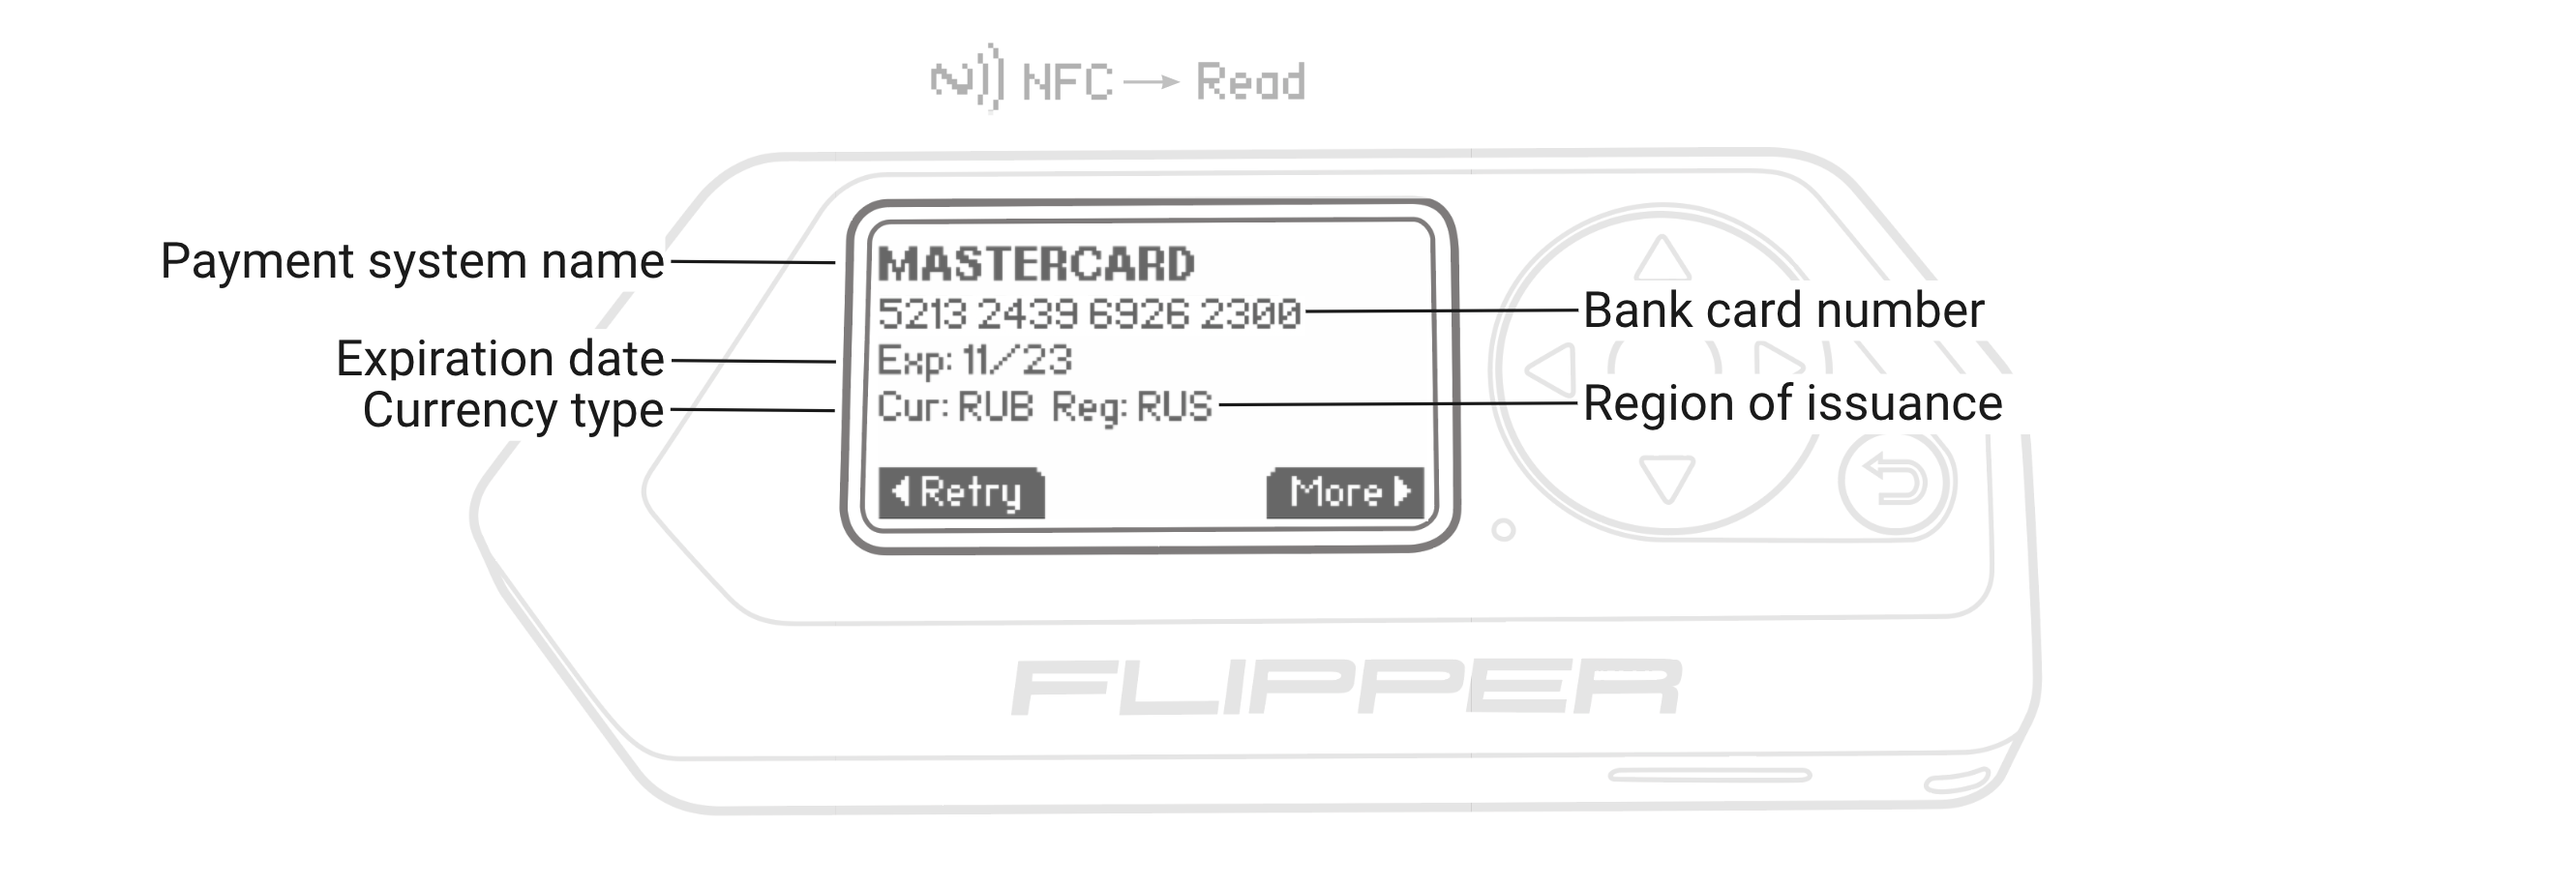
\includegraphics[width=.70\linewidth]{Bank_card.png}
	\label{fig:type.png}
\end{figure}

\textbf{Unknown cards} When Flipper Zero is unable to determine NFC card's type, then only an UID, SAK, and ATQA can be read and saved. Unknown card reading screenFor unknown NFC cards, Flipper Zero can emulate only an UID.

\begin{figure}[h]
	\centering
	\hspace{21pt}
	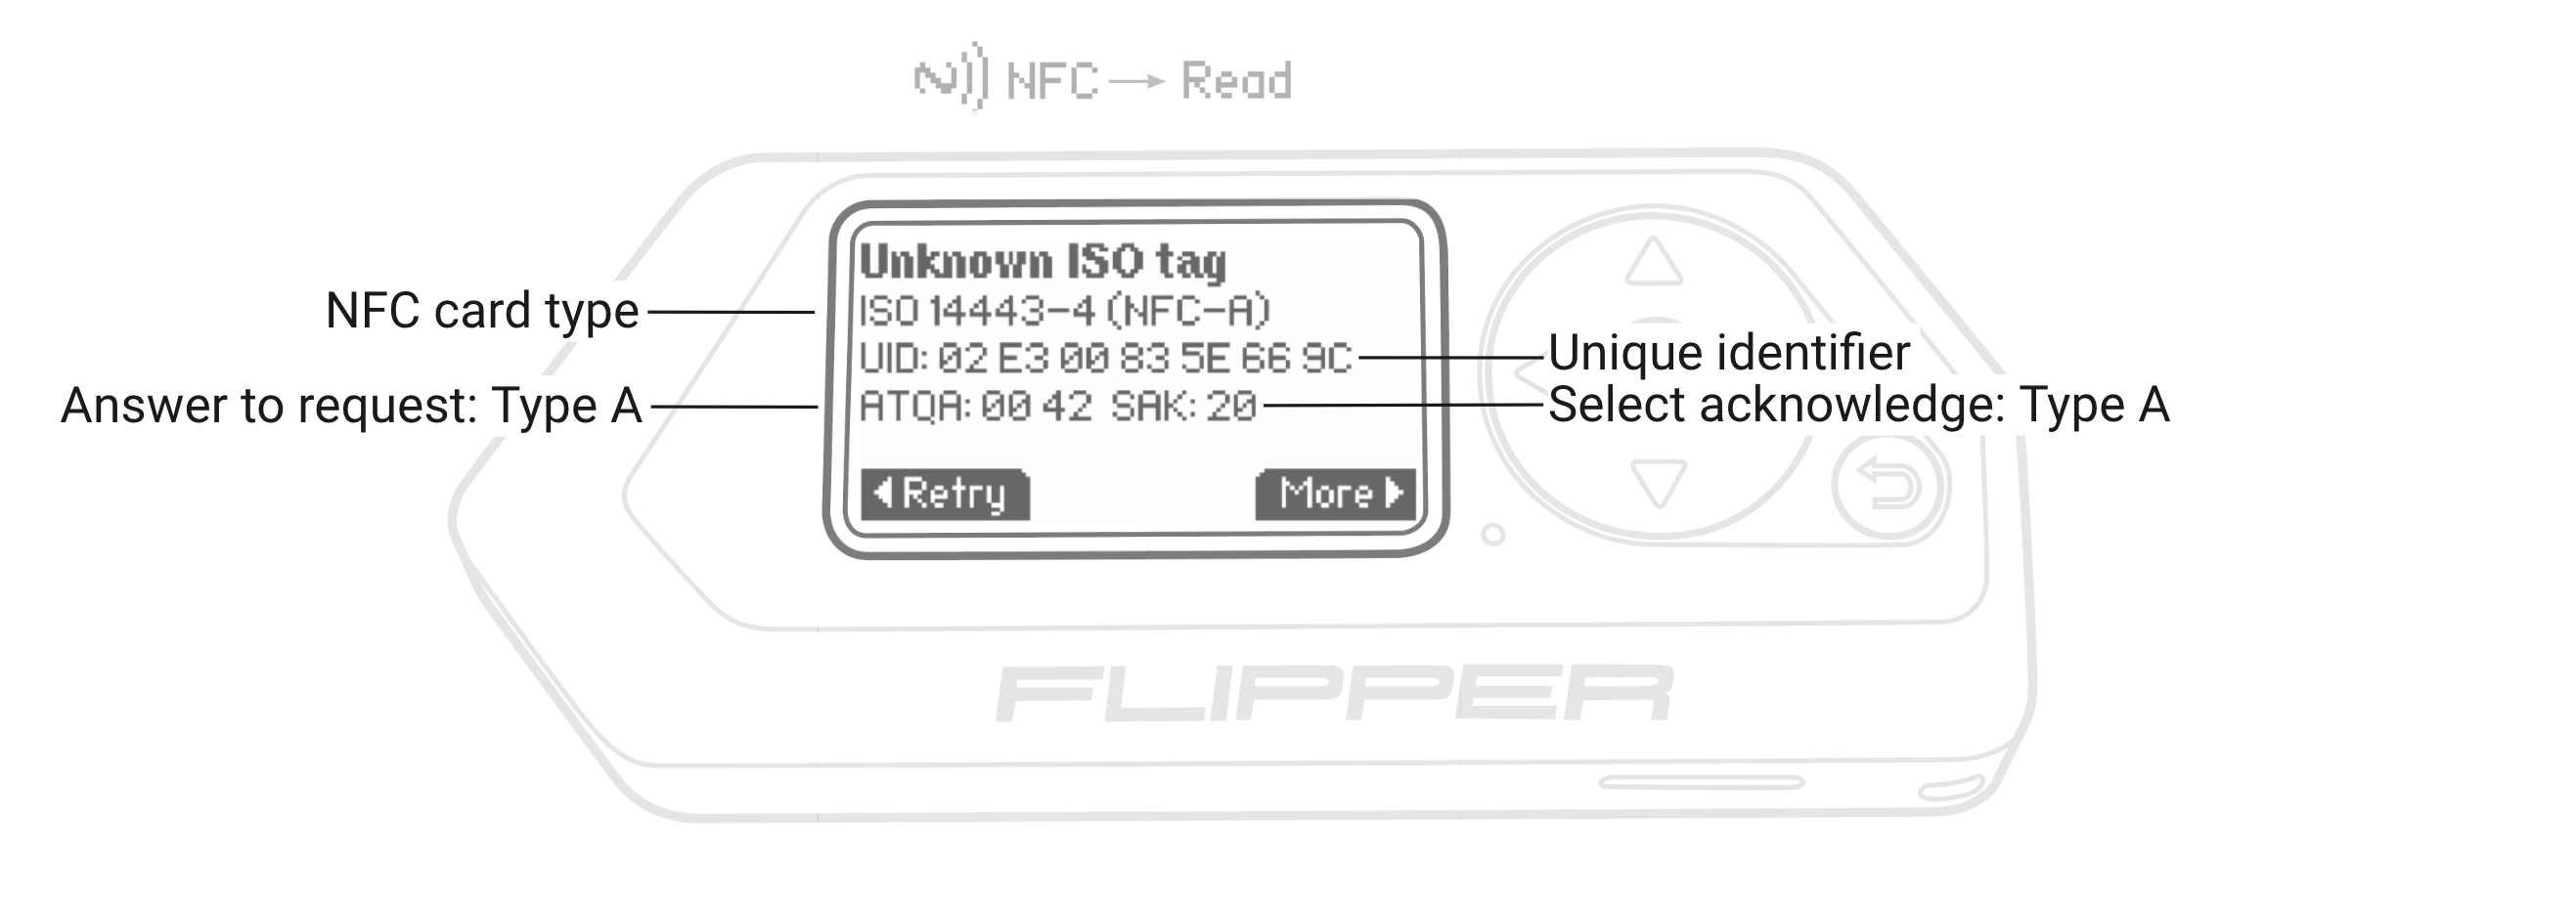
\includegraphics[width=.70\linewidth]{Unknown_card.png}
	\label{fig:type.png}
\end{figure}

\section{125kHz RFID}
RFID is a contactless radio-tag technology. It is quite common and you may see it in a lot of places: intercoms, bank cards, public transport passes, office passes, they are used to track domestic animals, for toll collection, etc. The two main RFID tag types are high frequency and low frequency.
\begin{itemize}
  \item \textbf{Low-Frequency tags (125 kHz)} — work at a higher range. Despite being insecure and dumb, they are still used in primitive access control systems: in building intercoms, offices, sports facilities, museums.
  \item \textbf{High-Frequency tags (13.56 MHz)} — have a lower effective range when compared with the low-frequency ones but have more complex protocols. They support encryption, authentication, and cryptography. These tags are commonly used in contactless bank cards, to pay for public transport, and in high-security access control systems.
  \end{itemize}
  \textbf{Popular 125 kHz protocols}
  
  \begin{itemize}
    \item \textbf{EM-Marin} — EM4100, EM4102. The most popular protocol in CIS. Can be read from about a meter because of its simplicity and stability. In this EM-Marin card in the physical card is possible to read the last 3 of 5 bytes in clear.
    The other 2 can be brute-forced if you cannot read them from the card.
  \end{itemize}

  \begin{figure}[h]
    \centering
    \hspace{21pt}
    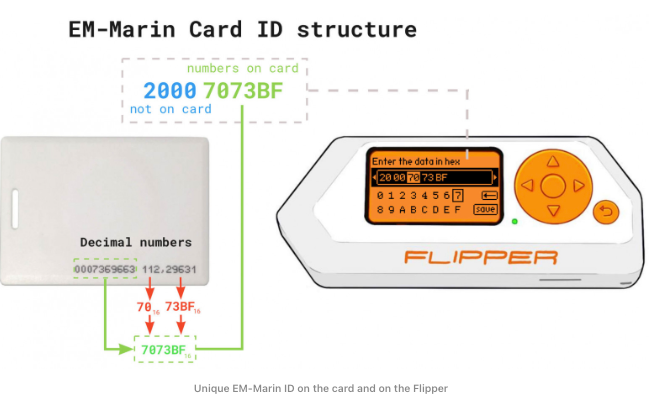
\includegraphics[width=.70\linewidth]{EM_marin.png}
    \label{fig:type.png}
  \end{figure}
  \begin{itemize}
    \item \textbf{HID Prox II} — low-frequency protocol introduced by HID Global. This protocol is more popular in the western countries. It is more complex and the cards and readers for this protocol are relatively expensive.
  \end{itemize}
  \begin{figure}[h]
    \centering
    \hspace{21pt}
    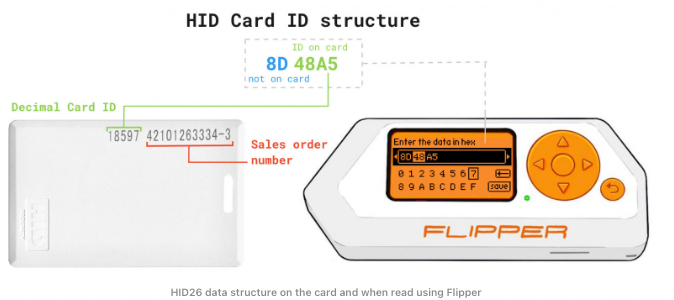
\includegraphics[width=.70\linewidth]{hid.png}
    \label{fig:type.png}
  \end{figure}
\section{Infrared}
\section{iButton}
\chapter{CONCLUSIONS}
Flipper Zero is a versatile, open-source hacking device that combines multiple features into a single device. It has a sleek and compact design, user-friendly interface, and numerous modules that can be added or removed based on users' needs. It can perform various hacking tasks, including sniffing, spoofing, jamming, cracking, and analyzing wireless protocols such as Bluetooth, Wi-Fi, NFC, and RFID. It has numerous potential applications in various fields, including cybersecurity, physical security testing, and IoT device testing. Overall, Flipper Zero is an excellent tool for security professionals, researchers, hobbyists, and enthusiasts who are interested in exploring and experimenting with wireless protocols and physical security testing.
\chapter{REFERENCES}
\begin{itemize}
\item [1] What is Flipper Zero INTRODUCTION  
                                                                     
https://flipperzero.one/
\item[2] A collection of Awesome resources for the Flipper Zero device.

https://github.com/djsime1/awesome-flipperzero
\item[3] Flipper zero Raradio-security

https://book.hacktricks.xyz/todo/radio-hacking/flipper-zero/
\vspace{12pt}
\end{itemize}
\end{document}
